\documentclass[12pt,a4paper]{article}
\usepackage[utf8]{inputenc}
\usepackage[spanish]{babel}
\usepackage{amsmath}
\usepackage{amsfonts}
\usepackage{amssymb}
\usepackage{graphicx}
\usepackage{hyperref}
\usepackage[left=2cm,right=2cm,top=3cm,bottom=3cm]{geometry}
\author{Rosario Collatón Chicana}
\title{Sesión 6}
\begin{document}
\maketitle
\tableofcontents
\listoffigures
\listoftables
\section{Introducción}
texto de la sección
\newpage
\section{Antecedentes}
texto de la sección
\newpage
\section{Metodología}
texto de la sección
\newpage
\section{Resultados}
Como podemos observar en el cuadro 
\ref{tab:result}

\begin{table}[h]
\centering
\begin{tabular}{|c|c|}
\hline 
1 & 2 \\ 
\hline 
2 & 3 \\ 
\hline 
\end{tabular} 
\caption{Tabla de los resultados}
\label{tab:result}
\end{table}
\newpage
También podemos observar en el gráfico
\begin{figure}[h]
\centering
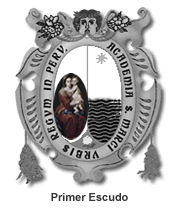
\includegraphics[scale=0.5]{UNMSM1}
\caption{Escudo de la UNMSM}
\end{figure}



\section{Discusión y conclusiones}
\end{document}